
To ensure the rocket has the ability to land, it must be sized to be feasible. Currently their are only a handful of proven rockets with the ability to vertically takeoff and land, these are from \textit{Space X} and \textit{Blue Origin}. To size reasonable parameters for the rocket, the \textit{Starship} launch vehicle from Space X shall be reviewed, this is a two stage launcher with the first stage called the \textit{Super Heavy Booster}, and a second stage called its namesake \textit{Starship}. The mass of each stage is shown in \autoref{tab:starship_parameters}, with their structural coefficients calculated through \autoref{eq:structural_coeff}. This launcher is able to carry 100-150 tonnes to LEO orbit, and 27 to GEO orbit (\cite{SpaceX2020_StarshipGuide}).

\begin{equation}
    \epsilon = \frac{m_s}{m_s + m_p}
\label{eq:structural_coeff}
\end{equation}

\begin{table}[htbp]
    \centering
    \caption{Mass and performance parameters of \textit{Super Heavy} and \textit{Starship}}
    \label{tab:starship_parameters}
    \begin{tabular}{@{}lcc@{}}
        \toprule
        & \textbf{Super Heavy booster} & \textbf{Starship} \\ \midrule
        Total mass [t]                          & 3,675 & 1,600 (excluding payload) \\
        Propellant mass [t]                     & 3,400 & 1,500 \\
        Structural mass [t]  & 275    & 100 \\
        Structural coefficient [-] & 0.0748 & 0.0625 \\ \bottomrule
    \end{tabular}
\end{table}

In terms of propellant, both stages use a fuel oxidiser mixture of liquid oxygen ($LOX$) and liquid methane ($LCH_4$) called methalox. The 2nd stage carries 1170 kg of $LOX$ and 330 kg $LCH_4$, giving a oxidiser-fuel ratio of 3.545; this is taken to be the same for the first stage too due to the same engines, Raptor 3, being used.


The Raptor 3 engines are top of the range full-flow cycle engines, with two varieties. One optimised for sea-level performance which is used on the 1st stage. The second is optimised for vacuum performance, with the 2nd stage taking 3 of these for ascent and 3 sea-level optimised engines for descent. From the specific impulse, a measure of rocket efficiency giving the thrust produced per unit flow of propellant, the exhaust velocities are calculated through \autoref{eq:exhaust_velocities}. As the engines are optimised for sea-level and vacuum, the nozzle exit pressures are assumed to be close to the pressure in those regimes to minimise the pressure losses, \autoref{eq:pressure_losses}. The parameters of the Raptor 3 engine variants are displayed in \autoref{tab:raptor3}.

\begin{equation}
    v_{ex} = I_{sp} \cdot g_0
\label{eq:exhaust_velocities}
\end{equation}

\begin{equation}
    T_{\text{pressure losses}} = (p_e - p_a) \cdot A_e
\label{eq:pressure_losses}
\end{equation}

\begin{table}[h!]
    \centering
    \caption{Parameters of the Raptor 3 engines}
    \label{tab:raptor3}
    \begin{tabular}{@{}lcc@{}}
        \toprule
        & \textbf{Sea-level Raptor 3 } & \textbf{Vacuum Raptor 3} \\ \midrule
        Specific impulse [s] & 350 & 380 \\
        Exit diameter [m] & 1.3 & 1.3 \\
        Exit area [$m^2$] & 1.327 & 2.3 \\
        Thrust [$MN$] & 2.745 & 2 \\
        Engine mass (integrated) [kg] & 1525 (1720) & 1525 (1720) \\
        Exhaust velocities [$m/s$] & 3433.5 & 3727.8 \\
        Exit pressure estimate [$kPa$] & 101 & 0 \\
        Engine Height [$m$] & 3.1 & 4.6 \\
        \bottomrule
    \end{tabular}
\end{table}


The thrust-to-weight ratio ($TWR$) is a crucial parameter affecting how much acceleration the rocket can produce, especially at take-off. The engines produce a certain thrust, resulting in the $TWR$ determining how many engines are on the rocket. The $TWR$ is calculated through \autoref{eq:TWR} to give the stage's $TWR$ in \autoref{tab:TWR}.

\begin{equation}
    TWR = \frac{T^e_i \cdot n^e_i}{m_i \cdot g_0}
\label{eq:TWR}
\end{equation}

\begin{table}[h!]
    \centering
    \caption{Stage's thrust-to-weight ratio.}
    \label{tab:TWR}
    \begin{tabular}{@{}lcc@{}}
        \toprule
        & \textbf{Super Heavy booster} & \textbf{Starship} \\ \midrule
        Number of engines [-] & 33 & 6 \\
        Stage Thrust-to-Weight ratio [-] & 2.51 & 0.7645 \\
        \bottomrule
    \end{tabular}
\end{table}

Space X's $TWR$ can be used to decide the number of engines on a different sized rockets. The TWR for each stage can be used to calculate the stage's maximum thrust, mass flow and number of engines from its initial mass by \autoref{eq:n_e}.


\begin{equation}
\begin{aligned}
    T^{req}_i =&  m_i(0) \cdot g_0 \cdot TWR_i\\
    n^e_i =& [\frac{T^{req}_i}{T^{engine}_i}] \\
    T^{max}_i =& n^e_i \cdot T^{engine}_i \\
    \dot{m}_i^{max} =& \frac{T^{max}_i}{v_{ex}^i}
\end{aligned}
\label{eq:n_e}
\end{equation}



%Resultingrocketwidthandgiballledetccc
\subsubsection{Number of engines}
The number of engines is used to size the width of the rocket, such that the rocket can fit the required number of engines. \autoref{fig:Raptor_Comparison} shows the layout of the Raptor engines for the Super Heavy Booster, they layour with 20 fixed engines in the outer ring, followed by an inner ring of 10 gimballed engines and a central triangle of gimballed engines, totalling in 20 fixed engines and 13 gimballed engines. Taking the three centrally gimballed engines as fixed independent of the rocket's configuration, the number of engines within the ring are altered, knowing that 2 extra outer ring engines are needed to fit one extra gimballed engines.

\begin{equation}
    r_r = r_{\text{superheavy}} \cdot (1 + \frac{n_{\text{outer}} - n_{\text{outer,superheavy}}}{n_{\text{outer,superheavy}}})
\end{equation}

\begin{figure}[H]
    \centering
    \begin{subcaptionbox}{Raptor 3 engine\footnotemark[1]\label{fig:Raptor_3}}[0.35\linewidth]
        {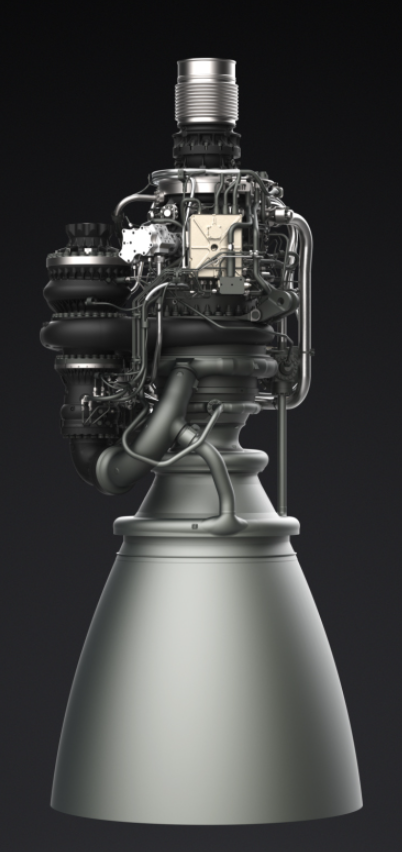
\includegraphics[width=\linewidth]{figures/LiteratureStudy/raptor_3.png}}
    \end{subcaptionbox}
    \hfill
    \begin{subcaptionbox}{Super Heavy engines\footnotemark[2]\label{fig:SuperHeavyEngines}}[0.58\linewidth]
        {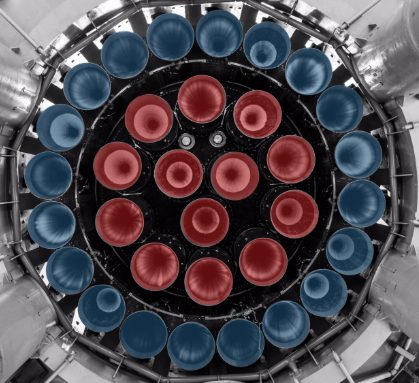
\includegraphics[width=\linewidth]{figures/LiteratureStudy/SuperHeavyRaptorLayour.png}}
    \end{subcaptionbox}
    \caption{Raptor 3 and Super Heavy engine layout}
    \label{fig:Raptor_Comparison}
    \footnotetext[1]{\url{https://www.spacex.com/vehicles/starship/}}
    \footnotetext[2]{\url{https://everydayastronaut.com/spacex-raptor-engine-comparison/}}
\end{figure}